\question
Найти для указанного графа и ДОПОЛНИТЕЛЬНОГО к нему:
\begin{enumerate}
\item  центр (отметить на графе);
\item  диаметр;
\item  радиус;
\item  три разных остовных дерева;
\item  цепь длиной 6 (покажите на графе);
\item  замкнутый путь длиной 10 (покажите на графе);
\item  вершинно-простой путь длиной 5 (покажите на графе);
\item  цикл длиной 4 и 6 (покажите на графе);
\item  простой цикл длиной 3 и 4 (покажите на графе);
\end{enumerate}
Примечание: для пунктов 5-9 рисуйте граф заново, если же выполнить уловие пункта задания невозможно  - обоснуйте 
\begin{figure}[h]

\begin{minipage}[h]{0.55\linewidth}
\end{minipage}
\begin{minipage}[h]{0.45\linewidth}
\center{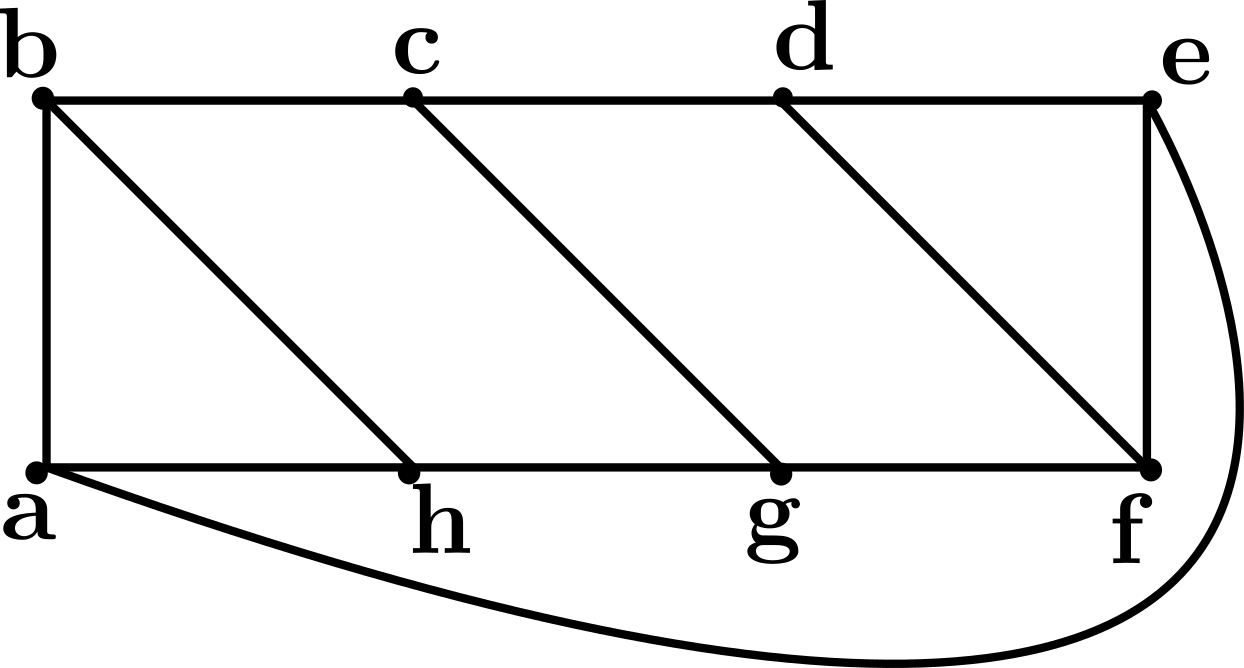
\includegraphics[width=0.6\textwidth]{pic/20.png}}
\end{minipage}
\end{figure}


